\documentclass[12pt]{beamer}

\usepackage[french]{babel}
\usepackage[T1]{fontenc}
\usetheme{metropolis}
\usepackage{booktabs}
\usepackage{tikz}
\usepackage{siunitx}
\sisetup{detect-weight=true, detect-family=true}

\urlstyle{same}  % Same font for URL as surrounding text

% Make footnotesize smaller
\makeatletter
\renewcommand\footnotesize{%
   \@setfontsize\footnotesize\@viipt{11}%
   \abovedisplayskip 8\p@ \@plus2\p@ \@minus4\p@
   \abovedisplayshortskip \z@ \@plus\p@
   \belowdisplayshortskip 4\p@ \@plus2\p@ \@minus2\p@
   \def\@listi{\leftmargin\leftmargini
               \topsep 4\p@ \@plus2\p@ \@minus2\p@
               \parsep 2\p@ \@plus\p@ \@minus\p@
               \itemsep \parsep}%
   \belowdisplayskip \abovedisplayskip
}
\makeatother


\title{Électricité et magnétisme}
\subtitle{Présentation du cours}
\date{24 août 2021}
\author{Loïc Séguin-Charbonneau}
\institute{Cégep Édouard-Montpetit}
% \titlegraphic{\hfill\includegraphics[height=1.5cm]{logo.pdf}}

\begin{document}
\setbeamertemplate{caption}{\raggedright\insertcaption\par}

\maketitle


\begin{frame}{Table des matières}
  \setbeamertemplate{section in toc}[sections numbered]
  \tableofcontents[hideallsubsections]
\end{frame}


\section{Pourquoi?}


%\begin{frame}[plain]{Combien d'êtres humains sur la planète?}
%  \begin{tikzpicture}
%    \node[align=right] (image) at (0, 0) {
%      \includegraphics[width=\textwidth]{images/crowd_james_cridland.jpg}
%      \\ \footnotesize \href{https://www.flickr.com/photos/jamescridland/613445810}{James Cridland}
%      (CC BY 2.0)
%    };
%    \only<2>{\node[rectangle, draw=orange!60, fill=orange!5, ultra thick,
%                   minimum height=3\baselineskip, minimum width=0.8\textwidth,
%                   fill opacity=0.8, text opacity=1, anchor=south,
%                   rounded corners, align=center]
%               at (image.center) {\Huge \alert{\textbf{\num{7 782 000 000}}}
%                 \\ \footnotesize \url{https://www.census.gov/popclock/world}};}
%  \end{tikzpicture}
%\end{frame}


%\begin{frame}{Quelle est l'aire de la Terre?}
%  \begin{columns}
%    \column{0.5\textwidth}
%    \begin{align*}
%      \onslide<2->{R &\approx \SI{6400}{km}}  \\
%      \onslide<3->{A &= 4 \pi R^2}  \\
%      \onslide<4->{A &\approx \SI{480e6}{km\squared}}
%    \end{align*}
%
%    \vspace{2cm}
%    \footnotesize
%    \onslide<2>{\url{https://nssdc.gsfc.nasa.gov/planetary/factsheet/earthfact.html}}
%
%    \column{0.5\textwidth}
%    \includegraphics[width=\textwidth]{images/earth.jpg}
%    \\ \footnotesize \href{https://www.flickr.com/photos/gsfc/6760135001/in/album-72157646899236025/}{NASA/NOAA/GSFC/Suomi NPP/VIIRS/Norman Kuring}
%  \end{columns}
%\end{frame}


\begin{frame}{Quelle aire de la planète par être humain?}
  \begin{columns}
    \column{0.5\textwidth}
    \includegraphics[width=\textwidth]{images/earth.jpg}
    \\ \footnotesize \href{https://www.flickr.com/photos/gsfc/6760135001/in/album-72157646899236025/}{NASA/NOAA/GSFC/Suomi NPP/VIIRS/Norman Kuring}
%    \begin{flalign*}
%      \onslide<1->{N &\approx \num{8e9}}  \\
%      \onslide<2->{A &\approx \SI{480e6}{km\squared}}  \\
%      \onslide<3->{\frac{A}{N} &\approx \frac{\SI{480e6}{km\squared}}{\num{8e9}}} \\
%      \onslide<4->{    &\approx \SI{60e-3}{km\squared}}  \\
%      \onslide<5->{    &\approx \SI{60000}{m\squared}}
%    \end{flalign*}

    \column{0.5\textwidth}
    \includegraphics[width=\textwidth]{images/kelly-sikkema-y9wY-3pi3-w-unsplash.jpg}
    \\ \hfill {\footnotesize \href{https://unsplash.com/photos/y9wY-3pi3-w}{Kelly Sikkema}}
    \pause
    
    \begin{tikzpicture}
    \node[rectangle, draw=orange!60, fill=orange!5, ultra thick,
          minimum height=3\baselineskip, minimum width=0.8\textwidth,
          fill opacity=0.8, text opacity=1, anchor=south,
          rounded corners, align=center]
          at (0, 0) {\Huge \alert{\textbf{\SI{60000}{m\squared}}}};
  \end{tikzpicture}
  \end{columns}
\end{frame}


\begin{frame}[plain]{Quelle aire par être humain?}
  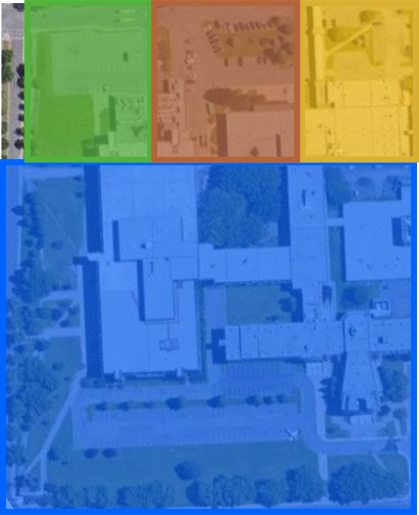
\includegraphics[width=\textwidth]{images/aire_par_habitant.jpg}
    \\ \footnotesize
    \hfill \href{https://www.google.ca/maps/@45.5358329,-73.4949587,489m/data=!3m1!1e3}{Google Maps}
\end{frame}


\begin{frame}[t]{Votre bout de Terre}
  % Eau : 71% de la surface terrestre
  %       (https://www.usgs.gov/special-topic/water-science-school/science/how-much-water-there-earth)
  % Déserts : 29% de la surface de terre ferme, incluant les glaciers (10%)
  %           (https://ourworldindata.org/agricultural-land-by-global-diets)
  % Forêts : 31% de la surface de terre ferme
  %          (http://www.fao.org/state-of-forests/en/)
  \definecolor{water}{RGB}{0, 99, 255}
  \definecolor{desert}{RGB}{217, 176, 50}
  \definecolor{forest}{RGB}{83, 178, 59}
  \definecolor{agriculture}{RGB}{178, 100, 59}

  \begin{columns}[T]
    \begin{column}{0.6\textwidth}

    \onslide<2->{\textcolor{water}{Eau (71\%)}
      \footnote<2->[frame]{\url{https://www.gsi.ie/en-ie/education/our-water/}}
    }

    \onslide<3->{\textcolor{desert}{Désert (29\% des terres)}
      \footnote<3->[frame]{
        \url{https://ourworldindata.org/agricultural-land-by-global-diets}
      }
      % Ce pourcentage inclut les glaciers.
    }

    \onslide<4->{\textcolor{agriculture}{Terres agricoles (36\% des terres)}
      \footnotemark[\value{footnote}]
      % Ce pourcentage est celui qu'on obtiendrait si tous les humains
      % adoptaient une diète semblable à celle de l'Espagne.
    }

    \onslide<5->{\textcolor{forest}{Forêt (31\% des terres)}
      \footnote<5->[frame]{\url{http://www.fao.org/state-of-forests/en/}}
      % Le pourcentage de forêts en 2021 est 31% des terres.
    }
    
    \vspace{\baselineskip}
    
    \onslide<6->{Il reste $\approx \SI{700}{m\squared}$}

    \end{column}

    \begin{column}{0.38\textwidth}

    \includegraphics<1>[width=\textwidth]{images/aire_par_habitant_1.png}
    \includegraphics<2>[width=\textwidth]{images/aire_par_habitant_2.png}
    \includegraphics<3>[width=\textwidth]{images/aire_par_habitant_3.png}
    \includegraphics<4>[width=\textwidth]{images/aire_par_habitant_4.png}
    \includegraphics<5->[width=\textwidth]{images/aire_par_habitant_5.png}
    \end{column}

  \end{columns}
\end{frame}


\begin{frame}{Et l'énergie?}
\begin{tikzpicture}
  \node[align=left] at (0, 4) {
    \footnotesize
    \href{https://commons.wikimedia.org/wiki/File:Hydro-energy.jpg}{Chalisa jirutchok}
    (CC BY-SA 4.0) \\
    \includegraphics[height=0.4\textheight]{images/dam.jpg}
  };
  \node[align=left] at (0, 0) {
    \includegraphics[height=0.4\textheight]{images/Belleville_nuclear_power_plant_and_two_pylons.jpg}
    \\ \footnotesize
    \href{https://commons.wikimedia.org/wiki/File:Belleville_nuclear_power_plant_and_two_pylons.jpg}{Cjp24}
    (CC BY-SA 4.0)
  };
  \node[align=right] at (5, 4) {
    \includegraphics[height=0.4\textheight]{images/panneau_solaire.jpg}
  };
  \node[align=right] at (5, 0) {
    \includegraphics[height=0.4\textheight]{images/wind_power.jpg}
    \\\footnotesize \hfill \href{https://www.flickr.com/photos/nualabugeye/753268301}{Nuala}
    (CC BY-NC-SA 2.0)
  };
  \node<2->[rectangle, draw=orange!60, fill=orange!5, ultra thick, align=center,
            minimum height=3\baselineskip, minimum width=0.5\textwidth,
            fill opacity=0.9, text opacity=1, anchor=south,
            rounded corners] at (2.5, 1.8)
            {\textbf{Il faut produire l'énergie efficacement} \\ \textbf{et l'utiliser intelligemment}};
\end{tikzpicture}
\end{frame}

\begin{frame}{Québec dans le monde}
  \begin{center}
  \includegraphics[width=0.9\textwidth]{images/comparaison-consommation-energetique.png}
  \end{center}
    \footnotesize
    {\href{https://energie.hec.ca/wp-content/uploads/2021/02/EEQ2021_web.pdf}{Whitmore, J. et P.-O. Pineau, 2021. État de l'énergie au Québec 2021,  
HEC Montréal.}}
\end{frame}

\begin{frame}{Quelle genre d'énergie est consommée?}
  \begin{center}
  \includegraphics[width=0.55\textwidth]{images/consommation-par-forme.png}
  \end{center}
    \footnotesize
    \hfill \href{https://energie.hec.ca/wp-content/uploads/2021/02/EEQ2021_web.pdf}{Whitmore, J. et P.-O. Pineau, 2021. État de l'énergie au Québec 2021,
     HEC Montréal.}
\end{frame}


\begin{frame}{Électrification des transports}
\begin{tikzpicture}
  \node[align=left] at (0, 4) {
    \footnotesize
    \href{https://commons.wikimedia.org/wiki/File:2018_Nissan_Leaf_Tekna_Front.jpg}{Vauxford}
    (CC BY-SA 4.0) \\
    \includegraphics[height=0.3\textheight]{images/nissan-leaf.jpg}
  };
  \node[align=left] at (0, 0) {
    \includegraphics[height=0.4\textheight]{images/chevrolet-bolt.jpg}
    \\ \footnotesize
    \href{https://commons.wikimedia.org/wiki/File:2019_Chevrolet_Bolt_EV_-_April_2019_(3165).jpg}{Gregory Varnum}
    (CC BY-SA 4.0)
  };
  \node[align=right] at (5, 4) {
  \footnotesize
    \href{https://commons.wikimedia.org/wiki/File:2019_Tesla_Model_3_Performance_AWD_Front.jpg}{Vauxford}
    (CC BY-SA 4.0) \\
    \includegraphics[height=0.3\textheight]{images/tesla-model-3.jpg}
  };
  \node[align=right] at (5, 0) {
    \includegraphics[height=0.4\textheight]{images/electric-bus.jpg}
    \\\footnotesize \hfill \href{https://commons.wikimedia.org/wiki/File:Electric_Bus.jpg}{Ryanmirjanic}
    (CC BY-SA 4.0)
  };
\end{tikzpicture}
\end{frame}



\begin{frame}{Comment réfléchir?}
  \begin{columns}
    \column{0.5\textwidth}
    \includegraphics[width=\textwidth]{images/membrane-potential.png}
    \\ \footnotesize \href{https://commons.wikimedia.org/wiki/File:Basis_of_Membrane_Potential2.png}{Synaptidude} (CC BY 3.0)

    \column{0.5\textwidth}
    \includegraphics[width=\textwidth]{images/cell-membrane-circuit.png}
    \\ \hfill {\footnotesize \href{https://commons.wikimedia.org/wiki/File:Cell_membrane_equivalent_circuit.svg}{Arne Nordmann, Looie496}
    (CC BY-SA 3.0)}
  \end{columns}
\end{frame}



\begin{frame}{Comment diagnostiquer?}
  \begin{columns}
    \column{0.5\textwidth}
    \includegraphics[width=\textwidth]{images/electrocardiogram.jpg}
    \\ \footnotesize \href{https://commons.wikimedia.org/wiki/File:2022_Electrocardiogram.jpg}{OpenStax College} (CC BY 3.0)


    \column{0.5\textwidth}
    \includegraphics[width=\textwidth]{images/mri.jpg}
    \\ \hfill {\footnotesize \href{https://commons.wikimedia.org/wiki/File:MRI-Philips.JPG}{Jan Ainali}
    (CC BY 3.0)}
  \end{columns}
\end{frame}

{
\usebackgroundtemplate{\includegraphics[height=\paperheight]{images/lightning.jpg}}%
\begin{frame}{S'émerveiller}
\color{black!40}
\begin{columns}
    \column{0.5\textwidth}
    \only<2>{
	  {
	    \color{black!10}
	    \begin{align*}
	      \oint \vec{\mathbf{E}} \cdot d\vec{\mathbf{A}} &= \frac{Q_\mathrm{int}}{\epsilon_0}  \\
		  \oint \vec{\mathbf{B}} \cdot d\vec{\mathbf{A}} &= 0  \\
		  \oint \vec{\mathbf{E}} \cdot d\vec{\mathbf{s}} &= -\int \frac{\partial\mathbf{B}}{\partial t} \cdot d\vec{\mathbf{A}} \\
		  \oint \vec{\mathbf{B}} \cdot d\vec{\mathbf{s}} &= \mu_0 I_\mathrm{int} + \frac{1}{c^2} \int \frac{\partial\mathbf{E}}{\partial t} \cdot d\vec{\mathbf{A}}
	    \end{align*}
	  }
	}
	\column{0.5\textwidth}
\end{columns}

\vskip0pt plus 1filll

\footnotesize \href{https://www.flickr.com/photos/snowpeak/14629877115/in/photolist-ohMWLB-8348WJ-8Yhdpt-2mfx7LV-8348LL-afKQP4-8348QL-2gY5QWX-9QDpw2-83491o-afNBbY-dRsJ7q-afNBbG-9QGfu7-9QwyuB-9KAZ8H-dezao9-QuVz-2bU2nXR-9DS4wj-agmf4L-awpe1q-7o2Qjr-mWt3L-MwWpo-6d6JZh-7vErDA-7wkrwj-6RDVrp-5vSgTT-dbSYbm-6jNdot-7w4prj-7wf2Km-7w4ptm-8hHWKp-7vunk6-Vr9vGL-aewo2i-2iAhwu-4M2gWV-cHXPF7-7jDZ18-59BnSF-nD6unu-i77q-6RDSWt-cCTJdY-8hHWDe-dcPoNZ}{John Fowler}
    (CC BY 2.0)
\end{frame}
}



\section{Quoi?}

% Carte des concepts au tableau.



\section{Qui?}

\begin{frame}{Un prof}
\begin{columns}
\column{0.5\textwidth}
Loïc Séguin-Charbonneau

\vspace{\baselineskip}

\onslide<2>{
Bureau D-1626

\vspace{\baselineskip}

Joignable par \textbf{mio} \\
Réponse en 24h (jours ouvrables seulement)
}

\column{0.5\textwidth}
\includegraphics[width=\textwidth]{images/lsc.jpg}

\end{columns}
\end{frame}


\begin{frame}{Disponibilités}
\begin{center}
\includegraphics[scale=0.5]{images/disponibilites.png}
\end{center}
\end{frame}


\begin{frame}{Vous autres}

\includegraphics[width=\textwidth]{images/students.jpg}

\end{frame}





\section{Comment?}

\begin{frame}{Avant les cours}
\begin{columns}
\column{0.6\textwidth}
Lire les sections du manuel indiquées dans le guide d'étude.

\vspace{\baselineskip}

\onslide<2>{Compléter le quiz de lecture en ligne.}

\column{0.4\textwidth}
\includegraphics[width=0.9\textwidth]{images/lafrance-em.jpg}

\end{columns}

\end{frame}


\begin{frame}{Pendant les cours}
\begin{columns}
\column{0.4\textwidth}
Retour sur les lectures

\vspace{\baselineskip}

\onslide<2->{Questions (feuille ABCD prêtée ou apportez la votre)}

\vspace{\baselineskip}

\onslide<3->{Résolution d'exercices}

\vspace{\baselineskip}

\onslide<4->{Laboratoires}

\column{0.6\textwidth}
\includegraphics[width=\textwidth]{images/teaching_physics.png}
\\ \footnotesize \url{https://xkcd.com/895}

\end{columns}

\end{frame}



\begin{frame}{Après les cours}
\begin{columns}
\column{0.6\textwidth}
Travailler sur les exercices spécifiés dans le guide d'étude

\vspace{\baselineskip}

\onslide<2->{Réviser la matière}

\vspace{\baselineskip}

\onslide<3->{Rédiger des rapports de laboratoire}

\column{0.4\textwidth}
\includegraphics[width=\textwidth]{images/resoudre.jpg}

\end{columns}

\end{frame}



\begin{frame}{Évaluations - Labos}
\begin{center}
\begin{tabular}{llc}
\toprule
\textit{Labo}  &  \textit{Titre}    &  \textit{Pondération}  \\
\midrule
1              & Loi d'Ohm          & 2\%                    \\
2              & Condensateurs      & 3\%                    \\
3              & Circuits cc        & Formatif               \\
4              & Pile réelle        & Formatif               \\
5              & Circuits RC        & 3\%                    \\
6              & Magnétisme         & 2\%                    \\
               & Devoirs, quiz, TP  & 5\%                    \\
               & Test labo          & 10\%                   \\
\bottomrule
\end{tabular}
\end{center}

\end{frame}



\begin{frame}{Évaluations - Examens}
\begin{center}
\begin{tabular}{lllc}
\toprule
\textit{Examen}  &  \textit{Date}    &  \textit{Chapitres}  &  \textit{Pondération}  \\
\midrule
1                &  28 septembre     & 1, 2, 3, 4           &  25\%                  \\
2                &  2 novembre       & 5, 6, 7, 12          &  25\%                  \\
3                &  À déterminer     & 8, 9, 10, 11, 12     &  25\%                  \\
\bottomrule
\end{tabular}
\end{center}

\end{frame}


\begin{frame}{Léa}
\begin{center}
\includegraphics[width=0.8\textwidth]{images/lea.png}
\end{center}
\end{frame}



\begin{frame}{C'est parti!}
Bon début de session!

On commence le chapitre 1 après la pause!
\end{frame}






\end{document}
